\chapter{Einleitung}
\markboth{1 Einleitung}{}

\section{Problemstellung}
%Unternehmen müssen aufgrund der heutigen dynamischen Veränderungen der Marktgegebenheiten die schnelle Entwicklung ihrer Produkte vorantreiben, sowie deren Platzierung und Bepreisung optimieren.\footnote{Vgl. \cite{gonsch2013using}, S. 94-95\label{dingens1}}
%Das Revenue Management (RM) ist daher für viele Dienstleistungsbereiche unabdinglich geworden. Durch dieses Managementkonzept und den daraus resultierenden Planungsinstrumenten können bei speziellen Anwendungsgebieten die Kapazitätsauslastungen optimiert werden. Damit lassen sich für Unternehmen mit Kapazitätsbe\-schränkungen die Absatzmärkte erfolgreich abschöpfen und die Gesamterlöse maximieren. In dieser Arbeit wird der Ansatz des Verkaufs von opaken Produkten im RM zur besseren Kapazitätsauslastung thematisiert. %\footnote{Klassische Ansätze des RM beschäftigen sich mit der Optimierung der Kapazitätsauslastung bei der Erstellung von Produkten oder Dienstleistungen.}
%Bei opaken Produkten handelt es sich um Produkte, bei denen der Anbieter einige Eigenschaften des Produkts bis zum Abschluss der Transaktion verbirgt.\footref{dingens1} %Anders als bei spezifischen Produkten, bei dem sämtliche Bestandteile der Produkteigenschaften vor dem Kauf bekannt sind.
%Die vorgestellten Produktarten werden i. d. R. in der Dienstleistungsindustrie von multiplen Anbietern angeboten.\footnote{Vgl. \cite{Klein:2008aa}, S. 4} Vereinfacht gesagt bedeutet dies, dass diese Anbieter ihre Dienstleistungen über eine Mehrmarkenstrategie distribuieren und ggf. ihr eigenes Produktportfolio mit anderen Dienstleistungen von Partnerfirmen erweitern. Sie bündeln aus dieser Menge an verfügbaren unterschiedlichen Dienstleistungen ein neues zusammenhängendes Produkt und vertreiben diese Art von Produkten über eine einzelne Marke an potentielle Konsumenten. Aus einem solchen Netzwerk an verfügbaren Produkten kann der Anbieter opake Produkte formen.\footnote{Vgl. \cite{anderson2009effectiveness}, S. 307-309}\textsuperscript{,}\footnote{Siehe Kapitel \ref{DP}}\\

Die Entscheidung über die Annahme von Kundenaufträgen hat weitreichenden Einfluss auf den Ertrag von produzierenden Unternehmen. Einem Unternehmen, dass zusätzlich zur Produktion die Instandsetzung ihrer Güter anbietet, stellt sich die Frage, ob eine Reparatur des Gutes wirtschaftlich ist. Im weiteren Verlauf dieser Arbeit werden diese Unternehmen als sogenannter Instandhalter bezeichnet. Abhängig des eingehenden Kundenauftrags, indem der Zustand des Gutes beschrieben ist, durch den die notwendigen Prozessschritte zur Instandsetzung des Gutes abgeleitet werden können, generiert der Dienstleister unterschiedliche Erträge. Diese Prozessschritte zur Instandsetzung des Gutes geben zusätzlich den notwendigen Ressourcenbedarf für die auszuführende Dienstleistung an, die notwendig sind um das Gut in seinen ursprünglichen bzw. geforderten Zustand zu versetzen. Ressourcen zur Instandsetzung von Gütern können z. B. Material oder Personalstunden sein. Abhängig des dadurch möglichen Ertrags und des für den Auftrag notwendigen Ressourcenbedarf muss das produzierende Unternehmen die Entscheidung über Annahme oder Ablehnung des Kundenauftrags treffen. Sofern nur der einfache Fall betrachtet wird, bei dem nur der einzelne Kundenauftrag zur Auswahl steht, ist die Entscheidung für den Instandhalter einfach getroffen. Der Kundenauftrag wird angenommen, sofern der Aufwand des Ressourceneinsatzes niedriger als der erziele Umsatz ist.
Sofern das Unternehmen eine begrenzte Ressourcenkapazität zur Instandsetzung der Güter besitzt, muss zusätzlich der absolute Ressourcenverbrauch des Auftrags für Annahmeentscheidung geprüft werden. Mit Annahme des Auftrags ist ein auftragsbezogener Ertrag erzielt und ein produktbezogener Ressourcenverbrauch eingetreten. Nachdem diese Entscheidung getroffen ist, wird der zeitlich darauffolgende Kundenauftrag betrachtet.

Für die Entscheidung über die Annahme oder Ablehnung eines Kundenauftrags (KA) zur Instandhaltung von Gütern bedarf es einer umfassenderen Betrachtung als nur die kurzsichtige Entscheidung über die Annahme einzelner Aufträge. Angenommen ein Instandhalter besitzt ein bestimmtes Kontingent an unterschiedlichen Ressourcen über einen bestimmten Zeitraum zur Erfüllung seiner angebotenen Dienstleistung. In diesem betrachteten Zeitraum treffen jetzt Kundenaufträge mit unterschiedlicher Wertigkeit ein. Zur Maximierung seiner Erträge über diesen Zeitraum kann es sinnvoll sein Anfragen mit niedrigem Ertrag abzulehnen, sofern im weiteren Verlauf des betrachteten Zeitraums Aufträge mit höherem Ertrag eintreffen. Dies erfolgt in Abhängigkeit der noch vorhanden knappen Ressourcenkapazität.

Eine weitere Alternative wäre es für das produzierende Unternehmen das zu reparierende Gut mit ein neuwertiges Gut auszutauschen. Es handelt sich damit um eine Entscheidung der Lagerentnahme. Die Entscheidung der Reduzierung des vorhandenen Lagerbestands zur Befriedung des Kundenauftrags macht vor allem Sinn, wenn die Reparatur des Auftrags mehr Kosten verursacht, als ein neuwertiges Gut in der Produktion kostet. Auch hier kann zwischen einer kurz- und langfristigen Sichtweise unterschieden werden. Die kurzfristige Sichtweise bezieht sich nur auf das Verhältnis zwischen Reparatur- und Produktionskosten des auftragsbezogenen Gutes. Bei der langfristigen Sichtweise wird der Lagerbestand über einen längeren Zeitraum betrachtet. Sofern in der nahen Zukunft viele Aufträge über neue Produkte eintreffen, ist es für das betrachtete Unternehmen ertragsmaximierender das Gut zu reparieren, damit alle Aufträge erfüllt werden.

%%Eine mögliche grafische Darstellungsform dieser Problemstellung erfolgt als sogenannter Entscheidungsbaum. Bei dem Entscheidungsbaum handelt es sich um ein gerichteten azyklischen Graphen. Abhängig der eintreffenden Anfragen, der vorhandenen Kapazitäten, der möglichen Entscheidungen und des betrachteten Zeithorizont hat der Entscheidungsbaum eine unterschiedliche Anzahl an Kanten und Knoten. Ein Knoten bildet jeweils einen neuen Zustand des Systems ab und eine Kante die mögliche Entscheidung in einen neuen Systemzustand zu gelangen.



\section{Zielsetzung}

In dieser Arbeit wird ein mathematischen Modell zur Annahmeentscheidung eines Auftrags zur Instandhaltung eines Gutes durch die Entscheidung über eine mögliche Reparatur oder der Entscheidung der Lagerhaltung getroffen. Durch Annahme der Entscheidung zur Lagerhaltung des defekten Gutes wird dieses in die Lagerhaltung des Reparaturdienstleisters übernommen und durch ein bereits repariertes Gut ausgetauscht. Das reparierte Gut entspricht den vom jeweiligen Auftrag geforderten Instandhaltungszustand. Anders formuliert bedeutet dies, dass das produzierende Unternehmen nicht nur die Entscheidungsmöglichkeit über die Instandsetzung des Gutes hat, sonder auch die Möglichkeit hat in Abhängigkeit des verfügbaren Lagerbestandes bereits reparierte Güter zur Befriedigung der Kundenaufträge zu verwenden.

Bei der Problemformulierung der Auftragsannahmeentscheidung bei auftragsbezogenen Instandhaltungsprozessen handelt es sich um ein stochastisch-dynamisches Optimierungsmodell. Das Optimierungsmodell muss demnach die Entscheidung treffen, ob die Auftragsannahme zur Instandsetzung des Gutes, die Lagerhaltung des defekten Gutes sowie die Herausgabe eines bereits reparierten Gutes oder die Ablehnung des Kundenauftrags erfolgen soll. Diese Entscheidung erfolgt in Abhängigkeit der verfügbaren restlichen Ressourcenkapazitäten, die zur Instandsetzung der Güter notwendig sind, des aktuell-vorhandenen Lagerbestandes der bereits reparierten Güter und der noch potentiell eintreffenden Anfragen zur Instandhaltung von Gütern.

Zur Formulierung des Problems wird das Konzept des Revenue Managements aufgegriffen. Es handelt sich ursprünglich um ein Konzept zur Auftragsannahme von freien Sitzplätzen von Passagierflugzeugen. Das Grundmodell wird zur Annahme von Kundenaufträgen bzw. -anfragen von Dienstleistungsunternehmen mit beschränkten Ressourcenkapazitäten verwendet. %kommt aus der wissenschaftlichen Betrachtung des Revenue Management .
Damit lässt sich die mathematische Darstellung des Optimierungsmodells der Auftragsannahme- und Lagerhaltungsentscheidungen bei auftragsbezogenen Instandhaltungsprozessen als \textit{dynamische Programmierung (DP}) formulieren.
Die Aufgabe des DP ist laut \cite{talluri2004theory} die Entscheidungsfindung zu unterstützen, damit der Gesamtertrag des Dienstleisters maximiert wird. Der Gesamtertrag wird bewertet in Geldeinheiten (GE). 

%Bei den betrachteten Ressourcen handelt es sich um zeitgebundene Ressourcen mit einer jeweiligen vordefinierten Ressourcenkapazität über den gesamten Zeithorizont. 

Die Zielsetzung der Arbeit ist demnach das Grundmodell des Revenue Managements zur Annahme von Kundenaufträgen mit der Möglichkeit der Entscheidung der Lagerhaltung der Güter zu erweitern. Zusätzlich zur konzeptionellen Darstellung des hier betrachteten Auftragsannehmeproblems wird ein Algorithmus entwickelt, welches vorformulierte Beispielszenarien exakt löst.  Damit lässt sich numerisch untersuchen, welche Möglichkeiten sich durch die Betrachtung einer Lagerhaltung in der Auftragsannahme von auftragsbezogenen Instandhaltungsprozessen für Unternehmen ergeben.

\section{Aufbau der Arbeit}

\begin{figure}[h!]
  \begin{center}
    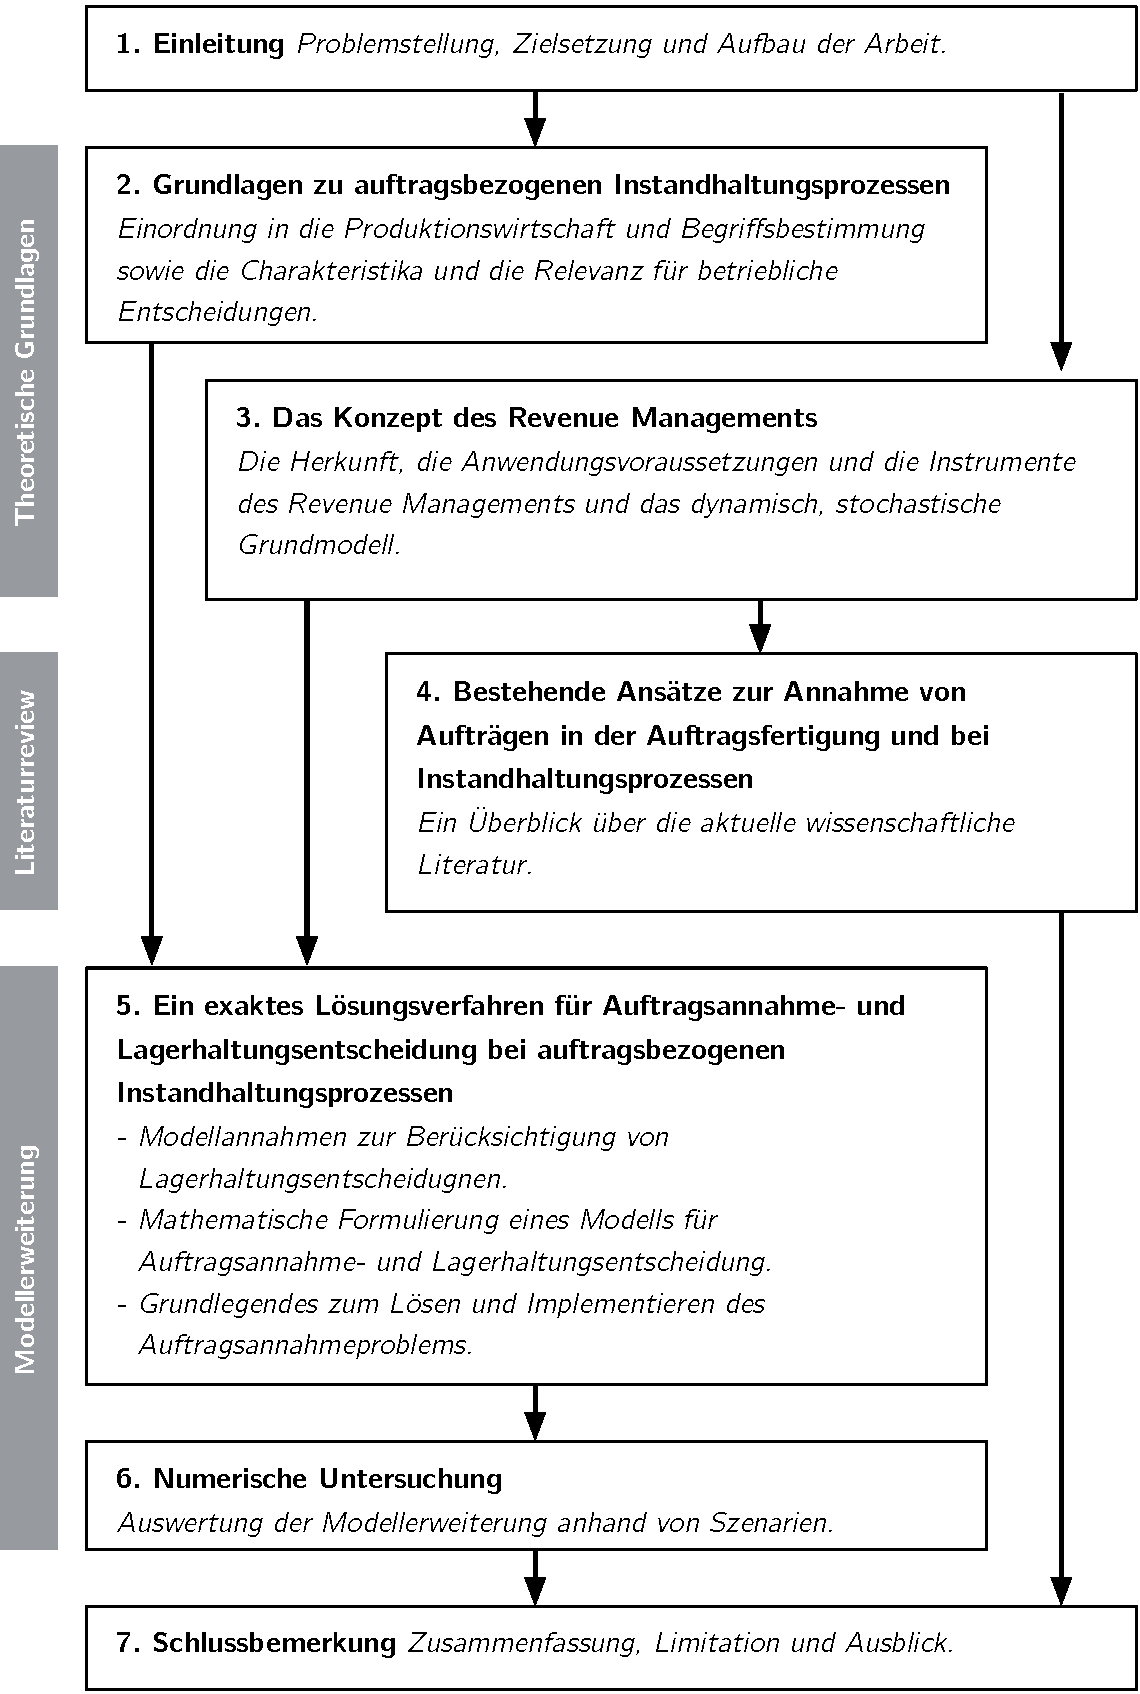
\includegraphics[width=140mm]{Bilder/Gliederung.pdf}
    \caption{Grafische Darstellung der Gliederung der Arbeit}  \label{Gliederung}
  \end{center}
\end{figure}


Der Aufbau der Arbeit ist in der Grafik \ref{Gliederung} dargestellt. Im Kapitel 2 wird vorerst der Begriff der auftragsbezogenen Instandhaltungsprozessen definiert und deren theoretische Grundlagen beschrieben. Der Begriff wird in diesem Kapitel in die Produktionswirtschaft eingeordnet, sowie die Charakteristika und die Relevanz für betriebliche Entscheidungen der auftragsbezogenen Instandhaltungsprozessen werden beschrieben. Weiter wird im Kapitel 3 die theoretischen Grundlagen der Arbeit vervollständigt, indem das Konzept des Revenue Management bei der Annahme von Aufträgen vorgestellt wird. In diesem Kapitel wird auf die Herkunft des Konzepts eingegangen. Für das Konzept bestehen Anwendungsvoraussetzungen und Instrumente, die in dem Kapitel beschrieben werden. Des Weiteren wird für das Grundmodell des Revenue Managements die mathematische Modellformulierung dargestellt.

Im Anschluss wird im Kapitel 4 ein Literaturüberblick über bestehende Ansätze zur Annahme von Auftragsproduktion und Instandhaltungsprozessen aufgeführt. Es werden hier vier Ansätze näher betrachtet, die den Fokus auf eine heuristische Lösung des Auftragsannahmeproblems legen.

Das Kapitel 5 zeigt die quantitative Untersuchung der Erweiterung des Grundmodells mit der Entscheidung über eine Lagerhaltung auf. Zum einen wird die  mathematische Modellformulierung und zum anderen wird ein Pseudo-Algorithmus zum exakten Lösen der Problemstellung beschrieben. Weiter werden die Grundlagen zur Implementierung des Pseudo-Alorithmus genannt. Im letzten Teil des Kapitels wird auf die numerische Untersuchung eingegangen.

Im letzten Kapitel sind die Schlussbemerkungen dieser Arbeit dargestellt. Es handelt dabei um eine Zusammenfassung und um einen Ausblick.